\documentclass[12pt]{article}
% ---------------------------------------------------------------- layout and fonts
\usepackage[a4paper,margin=2.54cm]{geometry}
\usepackage{fontspec}
% Times New Roman where installed (Windows, macOS, Overleaf); otherwise Liberation
% Serif, which has the same character widths, so line and page breaks match.
\IfFontExistsTF{Times New Roman}{\setmainfont{Times New Roman}}{\setmainfont{Liberation Serif}}
\usepackage{unicode-math}
\IfFontExistsTF{Times New Roman}{\setmathfont{Latin Modern Math}}{\setmathfont{Latin Modern Math}}
\usepackage{setspace}
\onehalfspacing
\usepackage[english]{babel}
\usepackage{csquotes}
\usepackage{microtype}
\usepackage{graphicx}
\usepackage{booktabs}
\usepackage{tabularx}
\usepackage{threeparttable}
\usepackage{caption}
\captionsetup{font={small,stretch=1.15},labelfont=bf,labelsep=period,justification=raggedright,singlelinecheck=false}
\usepackage{float}
\usepackage{amsmath}
\usepackage{enumitem}
\setlist{itemsep=2pt,topsep=4pt}
\usepackage{xcolor}
\definecolor{linkblue}{HTML}{1F4E9C}
\usepackage{titlesec}
\titleformat{\section}{\normalfont\large\bfseries}{\thesection}{0.6em}{}
\titleformat{\subsection}{\normalfont\normalsize\bfseries}{\thesubsection}{0.6em}{}
\titleformat{\subsubsection}{\normalfont\normalsize\bfseries\itshape}{\thesubsubsection}{0.6em}{}
\usepackage{fancyhdr}
\pagestyle{fancy}
\fancyhf{}
\renewcommand{\headrulewidth}{0pt}
\fancyhead[R]{\small\thepage}
\fancyhead[L]{\small STINT THEORY}

% ---------------------------------------------------------------- references (APA 7)
\usepackage[style=apa,backend=biber,uniquename=false]{biblatex}
\addbibresource{references.bib}

% ---------------------------------------------------------------- links
\usepackage[hidelinks=false,colorlinks=true,linkcolor=linkblue,citecolor=linkblue,urlcolor=linkblue,
  pdftitle={STINT THEORY: Does deep learning beat simpler models at forecasting Formula 1 lap times?},
  pdfauthor={Nahian Ibnat},bookmarksnumbered=true]{hyperref}
\usepackage[nameinlink,capitalise,noabbrev]{cleveref}
\crefname{equation}{Equation}{Equations}

% Make the whole author-date citation one link to its reference entry (not only the year).
\DeclareFieldFormat{citehyperref}{%
  \DeclareFieldAlias{bibhyperref}{noformat}%
  \bibhyperref{#1}}
\DeclareFieldFormat{textcitehyperref}{%
  \DeclareFieldAlias{bibhyperref}{noformat}%
  \bibhyperref{#1}}
\savebibmacro{cite}
\savebibmacro{textcite}
\renewbibmacro*{cite}{\printtext[citehyperref]{\restorebibmacro{cite}\usebibmacro{cite}}}
\renewbibmacro*{textcite}{\printtext[textcitehyperref]{\restorebibmacro{textcite}\usebibmacro{textcite}}}

\newcommand{\s}{\,s}
% \input is not expandable, so it breaks \bottomrule inside tables; use the primitive.
\makeatletter\newcommand\tabinput[1]{\@@input #1 }\makeatother

% table columns that wrap inside \textwidth
\newcolumntype{R}{>{\raggedleft\arraybackslash}X}
\newcolumntype{L}{>{\raggedright\arraybackslash}X}
% let long URLs break in the reference list
\setcounter{biburlnumpenalty}{100}
\setcounter{biburlucpenalty}{100}
\setcounter{biburllcpenalty}{100}


\begin{document}

% ======================================================================= title page
\begin{titlepage}
\centering
\vspace*{2.2cm}
{\Large\bfseries Does Deep Learning Beat Simpler Models at Forecasting\\[2pt] Formula~1 Lap Times?\par}
\vspace{0.6cm}
{\large Pre-registered tests, a tyre-age study and a strategy simulator,\\ 2023--2025\par}
\vspace{1.4cm}
{\large Nahian Ibnat\par}
\vspace{0.2cm}
{Independent Researcher\par}
\vspace{0.8cm}
{STINT THEORY research report\par}
\vspace{0.2cm}
{May 2026\par}
\vfill
\begin{minipage}{0.86\textwidth}
\small
\textbf{Data and code.} Lap timing from the OpenF1 interface \parencite{openf1}. Code, generated reports, pre-registrations
and the full log of model changes: \url{https://github.com/NahianIbnat-2000/stint-theory}. Interactive results and the
strategy simulator: \url{https://nahianibnat-2000.github.io/stint-theory/}.

\medskip
\textbf{Note on figures.} Every number, table and figure in this report is generated by code in the repository from
the stored result files; none is entered by hand.

\medskip
This is an independent research project. It is not affiliated with, or endorsed by, Formula~1, the FIA, Pirelli or
any team.
\end{minipage}
\end{titlepage}

% ======================================================================= abstract
\begin{abstract}
\noindent
This report asks whether deep learning forecasts Formula~1 lap times better than statistical and standard machine
learning models, and what the answer implies for race strategy. Using 76,814 driver-laps from 69 Grands Prix
(2023--2025), ten models were trained on earlier races and scored once on twelve locked test races, under comparisons
written down before the test data were opened. For the next lap, three neural networks (a multilayer perceptron, a
long short-term memory network and a temporal convolutional network) were statistically equivalent to gradient-boosted
trees within a pre-set margin of 0.01\,s per lap. All four cut the error of repeating the last lap by 12.3--12.7\%,
while the slowest network needed about 85 times the training time of the boosted trees. Over ten laps, boosted trees
reduced the error of the total by 1.02\,s against repeating the last lap and were slightly more accurate than the
recurrent network. A fixed-effects model of lap time on tyre age finds that each extra lap on a set is associated with
0.042--0.068\,s of lost pace, depending on the compound, once fuel burn and track changes are held fixed; without that
adjustment, the association disappears. A leave-race-out strategy simulator beats a naive forecast of post-stop pace by
45\% but is about 19\,s too slow over two thirds of a race, and its 90\% ranges cover only 74\% of real outcomes. A case
study of the 2024 Italian Grand Prix shows the simulator agreeing with the winning one-stop call while overstating its
margin. The evidence suggests that, for public timing data, more model complexity did not buy accuracy; the binding
limit appears to be information that no model sees.

\medskip
\noindent\textbf{Keywords:} Formula~1, forecasting, deep learning, gradient boosting, pre-registration, tyre degradation,
fixed effects, Monte Carlo simulation, race strategy
\end{abstract}

\newpage
{\singlespacing\tableofcontents}
\newpage

% ======================================================================= 1 introduction
\section{Introduction}\label{sec:intro}

A Formula~1 race strategy is a sequence of decisions about when to stop for new tyres and which tyres to fit. Each
stop costs time in the pit lane, and each lap on an older set costs pace; the strategist's task is to balance the two
over the race \parencite{bekker2009,heilmeier2020vse}. Teams support these decisions with race simulations, which
rely in turn on forecasts of how fast a car will lap in the coming laps \parencite{heilmeier2020mc,heilmeier2022}. If
better forecasts are available, better strategies should follow.

Deep learning has transformed forecasting with images, text and sound, but its advantage on tabular data is not
established. Large benchmark studies find that tree-based ensembles such as gradient boosting remain at least as
accurate as neural networks on medium-sized tables of features \parencite{grinsztajn2022,shwartzziv2022}, and the M5
forecasting competition was won with tree-based methods \parencite{makridakis2022}. Lap-time data sit between the two
worlds: each lap is a row of features (tyre age, compound, fuel, weather), but laps also form sequences within a
driver's race, which recurrent and convolutional networks are designed to exploit
\parencite{hochreiter1997,bai2018}.

This report therefore asks one central question: \emph{can deep learning models predict Formula~1 lap times and
tyre-related pace loss more accurately than statistical and standard machine learning models, and what does the answer
imply for strategy decisions?} It answers it in four parts:

\begin{enumerate}
  \item \textbf{Task 1, the next lap.} Ten models forecast each driver's next lap time and are compared on twelve
  locked test races under pre-registered rules (\cref{sec:t1}).
  \item \textbf{Task 2, the next ten laps.} The strongest models forecast a ten-lap horizon, the quantity a strategist
  adds up (\cref{sec:t2}).
  \item \textbf{Task 3, the tyre-age effect.} A fixed-effects regression estimates how lap time changes with tyre age
  once fuel burn and track changes are removed (\cref{sec:t3}).
  \item \textbf{A strategy simulator,} built from these estimates, is checked against real races
  (\cref{sec:sim}) and applied to a well-known strategic call at the 2024 Italian Grand Prix (\cref{sec:case}).
\end{enumerate}

The report makes three contributions. First, it compares the model families on the same laps with a pre-registered,
leakage-checked design, so that the result cannot be tuned after the fact \parencite{nosek2018,kapoor2023}. Second, it
separates tyre ageing from fuel burn, which public lap times mix together, using an identification argument stated in
full. Third, it publishes the strategy simulator together with measured errors and an interval calibration test,
rather than presenting simulated outcomes as observations.

The main findings, in brief: on the next lap, the neural networks are equivalent to gradient-boosted trees; over ten
laps, the boosted trees are slightly ahead; tyre ageing is clearly visible only after fuel effects are removed; and the
simulator gets the direction of a famous strategy call right while overstating its size.
\Cref{sec:background} defines the terms used throughout. \Cref{sec:data,sec:methods} describe the data and methods,
\cref{sec:t1,sec:t2,sec:t3,sec:sim} the results, \cref{sec:case} the case study, and
\cref{sec:discussion,sec:limits,sec:conclusion} the discussion, limitations and conclusions.

% ======================================================================= 2 background
\section{Background and definitions}\label{sec:background}

\subsection{Race strategy terms}\label{sec:terms-race}

\paragraph{Grand Prix, lap and stint.} A Grand Prix is a race over a fixed number of laps of a circuit. A \emph{stint}
is the run of consecutive laps a driver completes on one set of tyres; strategy is the choice of how many stints to
run, how long each is, and on which tyres \parencite{heilmeier2020vse}.

\paragraph{Tyre compound.} Pirelli supplies slick (dry-weather) tyres in several rubber compounds that trade grip
against durability; for each event it nominates three, labelled \emph{soft}, \emph{medium} and \emph{hard}, chosen to
suit the circuit \parencite{pirelli_tyres,pirelli_choice}. Because the same label can refer to a different compound at
different circuits, this report always uses the event-relative labels.

\paragraph{Two-compound rule.} In a dry race, each driver must use at least two different slick compounds, which
forces at least one pit stop \parencite{pirelli_tyres,f1_monaco_rule}. Two events in the sample had additional rules:
the 2023 Qatar Grand Prix limited each set to 18 laps \parencite{fia_qatar2023}, the 2025 Monaco Grand Prix required at
least three sets of tyres, and so at least two stops \parencite{f1_monaco_rule}, and the 2025 Qatar Grand Prix limited
each set to 25 laps \parencite{f1_qatar2025}. The simulator enforces all of these.

\paragraph{Pit stop and pit loss.} A pit stop is a visit to the pit lane to change tyres. Its \emph{pit loss} is the
time lost against staying on track, which includes the slower in-lap and out-lap as well as the stationary time
\parencite{heilmeier2020mc}. This report estimates it as the in-lap plus the out-lap minus two laps at the driver's
reference pace.

\paragraph{Safety car, virtual safety car and red flag.} After an incident, race control can neutralise the race by
deploying a safety car, which leads the field at reduced speed, declaring a virtual safety car, under which every
driver must slow to a set pace, or stopping the race with a red flag. Neutralisations make pit stops cheaper and are a
main source of randomness in strategy \parencite{heilmeier2020mc}.

\paragraph{Tyre degradation and graining.} Tyre degradation is the loss of performance as a tyre is used. One form of
it is \emph{graining}: a surface defect that forms when the compound is stressed beyond its limit and breaks into small
cracks, leaving a rough tread with less grip \parencite{pirelli_graining}. Public timing data do not observe the tyre
itself, only lap times; this report therefore speaks of lap-time changes \emph{associated with} tyre age, not of
measured wear.

\subsection{Forecasting and evaluation terms}\label{sec:terms-eval}

\paragraph{Persistence forecast.} The naive or persistence forecast predicts that the next value equals the last
observed value; it is the standard benchmark that any forecasting model must beat \parencite{hyndman2021}. Here it is
the driver's last clean lap in the current stint.

\paragraph{Mean absolute error and root mean squared error.} For forecasts $\hat y_i$ of outcomes $y_i$, the mean
absolute error (MAE) is $\frac1n\sum_i|\hat y_i-y_i|$ and the root mean squared error (RMSE) is
$\sqrt{\frac1n\sum_i(\hat y_i-y_i)^2}$ \parencite{hyndman2006}. The MAE is in the units of the data (seconds) and is not
dominated by a few large errors, which makes it the more interpretable average \parencite{willmott2005}; it is the
primary metric here. \emph{Bias} is the mean of $\hat y_i-y_i$.

\paragraph{Skill score.} The relative improvement over a benchmark, $1-\mathrm{MAE}_{\text{model}}/\mathrm{MAE}_{\text{persistence}}$,
the share of the benchmark's error a model removes \parencite{hyndman2006}.

\paragraph{Rolling-origin evaluation.} A forecast evaluation in which each test period is predicted by a model fitted
only on data from before it, and the origin then moves forward \parencite{tashman2000}. It mimics real use and prevents
the future from informing the past.

\paragraph{Leakage.} Information in the training or input data that would not be available at prediction time, which
makes out-of-sample accuracy look better than it is \parencite{kaufman2012,kapoor2023}.

\paragraph{Pre-registration.} Writing down the hypotheses, data and analysis plan before seeing the outcome data, so
that confirmatory tests cannot be adjusted after the results are known \parencite{nosek2018}.

\paragraph{Clustered bootstrap.} The bootstrap estimates the sampling distribution of a statistic by resampling the
data with replacement \parencite{efron1979}. When observations are correlated within groups, whole groups are resampled
instead \parencite{cameron2008}; here the groups are races, because laps of the same race share weather, track and
incidents.

\paragraph{Paired comparison.} Two forecasts are compared on the same observations through the difference of their
losses, which removes variation the two share \parencite{diebold1995}.

\paragraph{Holm correction.} A step-down procedure that controls the probability of at least one false rejection
across a family of tests by comparing ordered $p$-values with increasingly lenient thresholds \parencite{holm1979}.

\paragraph{Equivalence test.} A test of whether a difference is small enough to ignore: with a pre-set margin
$\delta$, equivalence is concluded when the $1-2\alpha$ confidence interval of the difference lies entirely within
$[-\delta,\delta]$, the two one-sided tests (TOST) procedure \parencite{schuirmann1987,lakens2017}.

\subsection{Model families}\label{sec:terms-models}

\paragraph{Ridge regression.} Least squares with a penalty on the squared size of the coefficients, which stabilises
estimates when features are correlated \parencite{hoerl1970}.

\paragraph{Linear mixed-effects model.} A regression with fixed effects shared by all units and random effects that
vary by unit (here by driver), estimated jointly \parencite{laird1982}; fitted with statsmodels
\parencite{seabold2010}.

\paragraph{Random forest.} An average of many decision trees, each grown on a bootstrap sample with a random subset of
features considered at each split \parencite{breiman2001}.

\paragraph{Gradient-boosted trees (XGBoost).} An ensemble in which trees are added one at a time, each fitted to the
remaining errors of the current ensemble, with regularisation of tree complexity \parencite{chen2016}.

\paragraph{Multilayer perceptron (MLP).} A feed-forward neural network of stacked layers of weighted sums and nonlinear
functions, trained by back-propagating errors \parencite{rumelhart1986}.

\paragraph{Long short-term memory network (LSTM).} A recurrent neural network whose gated memory cell lets it carry
information across long sequences \parencite{hochreiter1997}.

\paragraph{Temporal convolutional network (TCN).} A network of causal, dilated convolutions over a sequence, in which
each output depends only on present and past inputs \parencite{bai2018}.

\paragraph{Training terms.} The neural networks use the Huber loss, which is quadratic for small errors and linear for
large ones and so limits the pull of outliers \parencite{huber1964}; the AdamW optimiser, which separates weight decay
from the gradient update \parencite{loshchilov2019}; dropout, which randomly removes units during training to reduce
overfitting \parencite{srivastava2014}; and early stopping on held-out races \parencite{prechelt1998}. They are
implemented in PyTorch \parencite{paszke2019}; the other models use scikit-learn \parencite{pedregosa2011} and XGBoost.

\subsection{Related work}\label{sec:related}

\textcite{bekker2009} built a discrete-event simulation of Formula~1 races to plan strategies, validated on three races
of the 2005 season. \textcite{heilmeier2020mc} added probabilistic effects, such as accidents and safety cars, through
Monte Carlo simulation, and \textcite{heilmeier2020vse} trained neural networks to make the pit-stop decisions inside
such a simulation. These studies take lap-time models as given or calibrate them per race. The present report instead
asks how accurately lap times can be forecast from public data, compares model families under a pre-registered test,
and measures the error of the simulator that results. On the machine learning side, it adds a domain test to the
evidence that tree ensembles match or beat neural networks on tabular data
\parencite{grinsztajn2022,shwartzziv2022}.

% ======================================================================= 3 data
\section{Data}\label{sec:data}

\subsection{Source}
Lap times, sector times, tyre stints, pit stops, race-control messages, positions and weather come from OpenF1, a free,
community-run interface to Formula~1 timing data that is independent of Formula~1 and the FIA and provides history from
the 2023 season onward \parencite{openf1}. The sample covers the 2023, 2024 and 2025 seasons. Because the data belong to
Formula~1 and its partners, lap-level tables are not redistributed; the repository publishes only derived results.

\subsection{Construction and checks}
Each race was downloaded, rebuilt into one row per driver per lap, validated and cleaned. Safety-car, virtual
safety-car and red-flag periods were rebuilt from race-control messages; in-laps (the lap entering the pit lane) were
inferred as the lap before each out-lap; and deleted laps were read from the stewards' messages. No row was dropped:
laps were \emph{flagged} instead, and each analysis selects the laps it needs. A lap is \emph{clean green} if it is
not a pit lap, not run under a neutralisation or yellow flag, not the first lap, not deleted and not affected by rain.
Races with fewer than 90\% of the expected driver-laps recorded were excluded; this removed one race, the 2025 Miami
Grand Prix (55.8\% complete).

\begin{table}[htbp]
\centering
\caption{Sample by season}\label{tab:data}
\begin{threeparttable}
\small
\begin{tabularx}{\textwidth}{lRRRRRR}
\toprule
Season & Races listed & In sample & Driver-laps & Clean green laps & Clean share (\%) & Lap times present (\%)\\
\midrule
\tabinput{tables/t_data.tex}
\bottomrule
\end{tabularx}
\begin{tablenotes}\footnotesize
\item \textit{Note.} Source: the project's coverage report (\texttt{data/reports/coverage.json}), built from OpenF1
\parencite{openf1}. ``Clean green'' laps exclude pit laps, neutralised and yellow-flag laps, first laps, deleted laps
and wet laps.
\end{tablenotes}
\end{threeparttable}
\end{table}

\Cref{tab:data} shows the sample: 69 races, 76,814 driver-laps and 60,283 clean green laps. The clean share is stable
across seasons at 78--79\%, and lap times are present for more than 99\% of laps in every season, so data coverage is
not a plausible explanation for differences between seasons. In economic terms, about one lap in five is ``noisy
supply'' (pit laps, neutralisations, incidents) that a forecaster must either model or set aside; the models here set it
aside when scoring, which is why the results describe racing laps, not every lap.

% ======================================================================= 4 methods
\section{Methods}\label{sec:methods}

\subsection{Prediction target}\label{sec:target}
At the end of lap $t$, a model forecasts lap $t+1$ (Task~1) or laps $t+1,\dots,t+10$ (Task~2) for a driver who stays out
on the same tyres. Forecasts are scored only on clean green target laps. Except for persistence, models predict the
change from a \emph{reference pace}: the driver's last clean lap in the current stint, or, early in a stint, the median
lap of other drivers in the previous two minutes. This keeps the large differences between circuits out of the
problem. All inputs are built only from information available at the end of lap $t$; an automated test perturbs future
laps and checks that no input changes, and a second test confirms that the first test detects a deliberately leaky
feature \parencite{kaufman2012}.

\subsection{Validation design}\label{sec:design}
The split was fixed before any model was fitted: the 2023 and 2024 seasons for training, with hyperparameters tuned
only inside 2024; the first half of 2025 (rounds 1--12) for development; and the second half of 2025 (rounds 13--24)
as the test set. Development and test both use rolling origins: each race is predicted by models trained on every
earlier race \parencite{tashman2000}. The test set was locked in code, every opening was logged, and each task was
scored on it once, after all models were frozen and the comparisons, margins and decision rules had been committed to
the repository \parencite{nosek2018}. The commit identifiers and file hashes are listed in \cref{app:repro}.

\subsection{Models}\label{sec:models}
Task~1 compares ten models (\cref{sec:terms-models}): persistence; \emph{compound drift} (persistence plus the average
lap-to-lap change for the compound in training); ridge regression; a linear mixed-effects model with a random intercept
and tyre-age slope by driver; a random forest; XGBoost; XGBoost averaged over five random seeds; and three neural
networks. The tabular models and the MLP see the same inputs: tyre age and its square, laps remaining (a fuel proxy),
weather, recent pace summaries (last clean lap, three-lap mean, five-lap spread and trend), field pace, compound,
circuit and team. The LSTM and TCN add the raw sequence of the driver's last ten laps. This design isolates two
questions: MLP against XGBoost compares learners on identical inputs, and LSTM or TCN against MLP measures what the raw
sequence adds. Neural networks were trained with five seeds and their predictions averaged, so the fair tree
comparator is XGBoost averaged over five seeds.

\subsection{Decision rules}\label{sec:rules}
Models are compared in pairs on the same laps through the difference in MAE \parencite{diebold1995}, with 95\% and
90\% race-clustered bootstrap intervals over 2,000 resamples \parencite{cameron2008}. For Task~1, five primary
comparisons and a practical margin of $\delta=0.01$\,s per lap were pre-registered. A comparison is labelled
\emph{equivalent} when the 90\% interval lies inside $\pm\delta$ (TOST at 5\%; \cite{lakens2017}), \emph{meaningful
difference} when the 95\% interval excludes zero and the whole 90\% interval lies beyond $\delta$, \emph{statistically
different, size unclear} when the 95\% interval excludes zero but the 90\% interval crosses the margin, and
\emph{inconclusive} otherwise. $p$-values are Holm-corrected across the primary family \parencite{holm1979}. Task~2
uses the same rules on the ten-lap total with $\delta=0.1$\,s.

\subsection{Task 3: the tyre-age effect}\label{sec:t3method}
Lap time $y_{irl}$ of driver $i$ in race $r$ on lap $l$, on compound $c$ with tyre age $a$, is modelled as
\begin{equation}\label{eq:fe}
  y_{irl} = \beta_{c}\,a_{irl} + \lambda_{rl} + \mu_{ir} + \kappa_{rc} + \varepsilon_{irl},
\end{equation}
where $\lambda_{rl}$ is a race-by-lap effect that absorbs everything common to all cars on a lap (fuel burn, track
evolution, wind), $\mu_{ir}$ a driver-by-race effect (car and driver pace at that event), and $\kappa_{rc}$ a
race-by-compound effect (the pace level of each compound at that event). $\beta_c$ is the lap-time change associated
with one more lap of tyre age on compound $c$. The model is estimated on clean green dry laps on slicks with the three
sets of fixed effects removed by alternating projections \parencite{guimaraes2010,gaure2013}, and standard errors are
clustered by race \parencite{cameron2015}.

Identification needs care. Within a stint, tyre age rises one-for-one with the lap number, so it cannot be separated
from $\lambda_{rl}$ by within-stint variation alone; this is a form of the age--period--cohort problem
\parencite{fosse2019}. The slope is identified from the pace change at a pit stop, when tyre age resets but the lap
number does not, compared across drivers who stopped at different ages. It therefore rests on two assumptions: a
driver's underlying pace is the same across stints within a race, and compound offsets are common to all cars at a
race. Replacing driver-by-race with driver-by-stint effects makes $\beta_c$ unidentified, and the code checks and
reports this. The estimates are associations, not causal effects of tyre wear: pit timing is chosen by teams, and
tyre management may differ by stint \parencite{angrist2009}.

\subsection{The strategy simulator}\label{sec:simmethod}
The simulator plays out the rest of a race for one car from a decision lap $L$, for any plan of stop laps and
compounds. Expected lap time on lap $j$ is
\begin{equation}\label{eq:sim}
  \mathbb{E}[y_j] = \mu + \beta\,j + \kappa_{c} + s_{\text{circuit}}\,\beta_{c}\,a_j ,
\end{equation}
with the tyre-age slopes $\beta_c$ from \cref{eq:fe}, compound offsets $\kappa_c$ estimated from same-lap comparisons
of cars on different compounds, a common per-lap trend $\beta$, and a circuit factor $s_{\text{circuit}}$ from other
years at the same circuit, normalised to average one. Every parameter is estimated \emph{without} the race being
simulated (leave-race-out). The driver's pace level $\mu$ comes only from laps already run. Lap-to-lap noise follows a
first-order autoregressive process, pit loss is drawn around the circuit's historical mean, and safety cars arrive at
the historical rate. Each plan is simulated 1,000 times with \emph{common random numbers}: every plan faces the same
draws, so differences between plans are not driven by luck \parencite{law2015,glasserman2003}. Normal draws use the
Box--Muller method \parencite{box1958}. The best plan for each number of stops is found exactly by dynamic programming
over stop laps and compounds \parencite{bellman1957}, under the tyre rules in \cref{sec:terms-race}. The simulator is a
single car against the clock: it models race time, not finishing positions, traffic or other cars' strategies.

% ======================================================================= 5 results
\section{Task 1: the next lap}\label{sec:t1}

\Cref{tab:t1} reports every model on the 11,041 scored laps of the twelve test races.

\begin{table}[htbp]
\centering
\caption{Next-lap forecasts on the locked test races}\label{tab:t1}
\begin{threeparttable}
\footnotesize
\begin{tabularx}{\textwidth}{Llrlrrrr}
\toprule
Model & Family & MAE (s) & 95\% CI & RMSE (s) & Bias (s) & Skill (\%) & Training (s)\\
\midrule
\tabinput{tables/t_task1.tex}
\bottomrule
\end{tabularx}
\begin{tablenotes}\footnotesize
\item \textit{Note.} 2025 rounds 13--24; 11,041 clean green laps; every model predicts the same laps. CI: race-clustered
bootstrap, 2,000 resamples \parencite{cameron2008}. Skill: share of the persistence forecast's MAE removed
\parencite{hyndman2006}. Training: seconds of fitting summed over the twelve test folds on one machine. Source:
\texttt{research/results/final\_test}.
\end{tablenotes}
\end{threeparttable}
\end{table}

Five models form a tight group: XGBoost averaged over five seeds, the LSTM and the TCN (MAE 0.333\,s each), single
XGBoost (0.334\,s) and the MLP (0.335\,s). Each removes about 12.3--12.7\% of the persistence forecast's error, which
is 0.382\,s. In plain terms, the typical miss on the next lap falls from about 0.38\,s to about 0.33\,s, roughly half a
tenth of a second. The random forest is close behind; ridge regression removes 5.8\%, compound drift almost nothing,
and the mixed-effects model is 2.2\% \emph{worse} than persistence, a reminder that adding driver-specific structure
does not help when the extra parameters are noisy. The confidence intervals of the models overlap heavily, but they
describe race-to-race uncertainty that all models share; the paired comparisons below remove it.

\begin{table}[htbp]
\centering
\caption{Pre-registered primary comparisons, next lap}\label{tab:p1}
\begin{threeparttable}
\footnotesize
\begin{tabularx}{\textwidth}{lLrllrl}
\toprule
& Comparison & $\Delta$MAE (s) & 90\% CI & 95\% CI & Holm $p$ & Label\\
\midrule
\tabinput{tables/t_primary1.tex}
\bottomrule
\end{tabularx}
\begin{tablenotes}\footnotesize
\item \textit{Note.} $\Delta$MAE is the first model's MAE minus the second's on the same laps; negative favours the first
model. Equivalence margin $\pm$0.01\,s per lap, fixed in the pre-registration (\cref{app:repro}); labels as defined in
\cref{sec:rules} \parencite{lakens2017}. Holm correction over the five comparisons \parencite{holm1979}.
\end{tablenotes}
\end{threeparttable}
\end{table}

\begin{figure}[htbp]
\centering
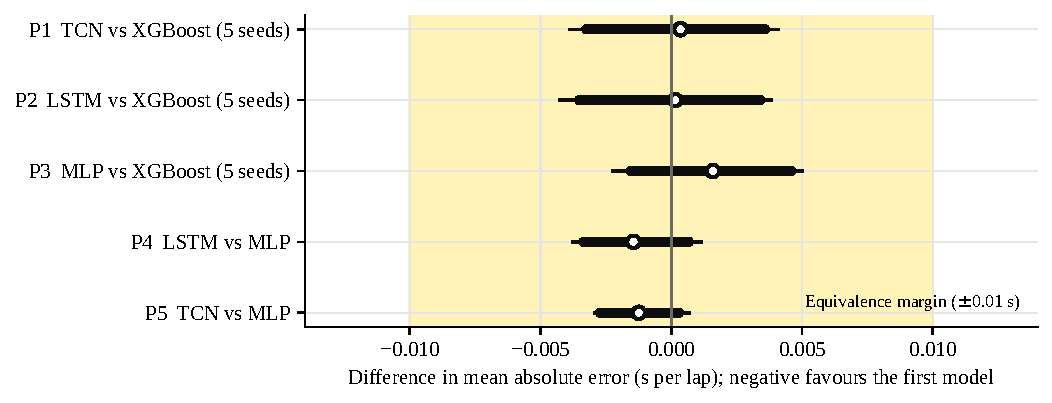
\includegraphics[width=\textwidth]{figures/f_primary1.pdf}
\caption{Pre-registered comparisons with 90\% (thick) and 95\% (thin) race-clustered intervals. The shaded band is the
equivalence margin. Source: \cref{tab:p1}.}\label{fig:p1}
\end{figure}

All five pre-registered comparisons are \emph{equivalent} (\cref{tab:p1,fig:p1}): every 90\% interval lies inside
$\pm$0.0046\,s, less than half the margin. The largest point difference, MLP against XGBoost, is 0.0016\,s per lap,
about 3\% of the 0.049\,s that separates XGBoost from persistence. None is close to statistical significance after
correction (smallest Holm $p$ = 0.93). Race by race, the networks beat the averaged XGBoost in only four or five of the
twelve test races, which is what equal accuracy would produce.

Two further results shape the interpretation. First, cost: the TCN needed 6,480\,s of training against 76\,s for the
averaged XGBoost and 16\,s for a single XGBoost (\cref{tab:t1}), about 85 and 400 times as much, for no gain. Seen as an
investment, the marginal return on model complexity here is close to zero. Second, randomness: retraining the same
network with another seed moves its MAE by a standard deviation of 0.0014--0.0016\,s, which is as large as the
differences between architectures; architecture choice is lost in the noise of initialisation.

\begin{figure}[htbp]
\centering
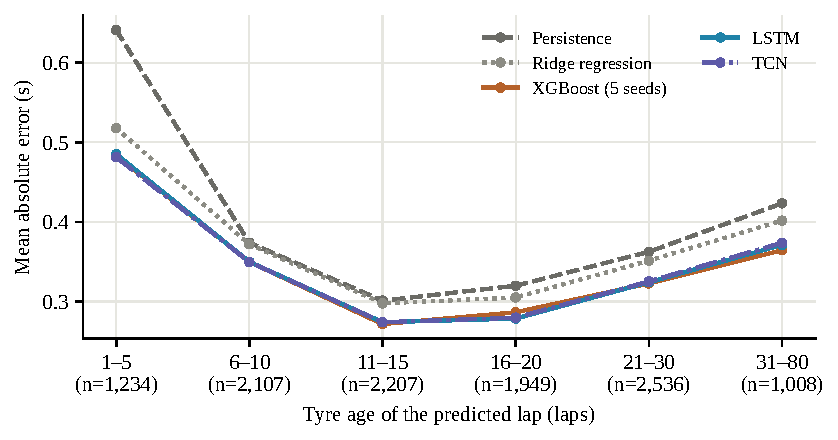
\includegraphics[width=\textwidth]{figures/f_tyreage_error.pdf}
\caption{Mean absolute error by tyre age of the predicted lap, test races. Descriptive breakdown of the single test run;
no intervals. Source: \texttt{research/results/final\_test}.}\label{fig:tyreerr}
\end{figure}

Where are the forecasts hardest? \Cref{fig:tyreerr} shows that errors are highest in the first five laps of a stint
(0.48\,s for the best models, 0.64\,s for persistence), lowest for tyres 11--15 laps old (0.27\,s) and rise again beyond
30 laps (0.36\,s). Fresh tyres warm up and settle in ways the inputs describe poorly, and very old tyres are rarer and
less predictable. On those old tyres, a secondary analysis that was not corrected for multiple testing finds the TCN
worse than the averaged XGBoost by 0.009\,s per lap (95\% CI 0.003 to 0.015, 1,008 laps), the one place where a network
fell measurably behind.

% ----------------------------------------------------------------------- Task 2
\section{Task 2: the next ten laps}\label{sec:t2}

A strategist needs pace over the coming laps, not one lap. Task~2 forecasts laps $t+1$ to $t+10$ and scores the error of
their total, on 5,241 forecast origins whose ten laps were all scored.

\begin{table}[htbp]
\centering
\caption{Ten-lap forecasts on the locked test races}\label{tab:t2}
\begin{threeparttable}
\small
\begin{tabular}{lrr}
\toprule
Model & MAE of 10-lap total (s) & Bias (s)\\
\midrule
\tabinput{tables/t_task2_models.tex}
\bottomrule
\end{tabular}
\smallskip

\footnotesize
\begin{tabularx}{\textwidth}{lLrll>{\raggedleft\arraybackslash}p{1cm}>{\raggedright\arraybackslash}p{2.6cm}}
\toprule
& Comparison & $\Delta$MAE (s) & 90\% CI & 95\% CI & Holm $p$ & Label\\
\midrule
\tabinput{tables/t_primary2.tex}
\bottomrule
\end{tabularx}
\begin{tablenotes}\footnotesize
\item \textit{Note.} 5,241 origins in 12 races. Equivalence margin $\pm$0.1\,s on the ten-lap total, pre-registered
separately for Task~2 (\cref{app:repro}). Settings were carried over from Task~1 without retuning; the TCN was left out
because it matched the LSTM in Task~1 at twice the cost. Source: \texttt{research/results/task2\_test}.
\end{tablenotes}
\end{threeparttable}
\end{table}

\begin{figure}[htbp]
\centering
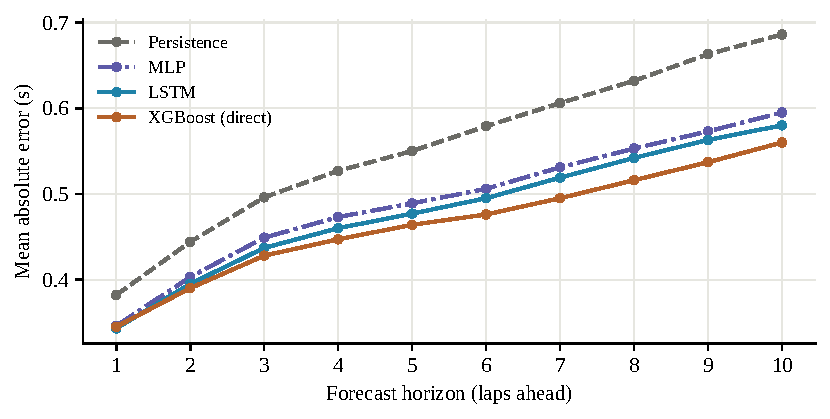
\includegraphics[width=\textwidth]{figures/f_horizon.pdf}
\caption{Mean absolute error by forecast horizon, test races. Source: \texttt{research/results/task2\_test}.}\label{fig:horizon}
\end{figure}

XGBoost, fitted directly to all ten horizons, is the most accurate (\cref{tab:t2}). It cuts the error of the ten-lap
total from 4.36\,s for persistence to 3.34\,s, a reduction of 1.02\,s (95\% CI 0.69 to 1.27), or 23\%; this is a
meaningful difference under the pre-registered rule. To put the size in context, a pit stop costs about 25\,s
(\cref{sec:sim}), so better forecasting removes about 4\% of the price of a stop from the uncertainty over the next ten
laps. The LSTM is behind XGBoost by 0.135\,s (95\% CI 0.030 to 0.270; Holm $p$ = 0.016): statistically different, but
with the 90\% interval crossing the 0.1\,s margin its practical size is unclear. At about half a percent of a pit stop,
it is unlikely to change a strategy. The raw lap sequence again adds little: LSTM against MLP is inconclusive.
\Cref{fig:horizon} shows the gap to persistence widening with the horizon, from 0.04\,s at one lap to 0.13\,s at ten:
the value of a model, like compound interest, accumulates over the laps it is asked to look ahead. Forecast errors of
the same origin are strongly correlated across the ten laps (0.68 for XGBoost), so errors do not average out over a
stint; the simulator models this with autocorrelated noise.

% ----------------------------------------------------------------------- Task 3
\section{Task 3: the tyre-age effect}\label{sec:t3}

\begin{table}[htbp]
\centering
\caption{Lap-time change per extra lap of tyre age (s), with 95\% intervals}\label{tab:t3}
\begin{threeparttable}
\footnotesize
\begin{tabularx}{\textwidth}{>{\raggedright\arraybackslash}p{4.4cm}LLL}
\toprule
Specification & Soft & Medium & Hard\\
\midrule
\tabinput{tables/t_task3.tex}
\bottomrule
\end{tabularx}
\begin{tablenotes}\footnotesize
\item \textit{Note.} Estimates of $\beta_c$ in \cref{eq:fe}; clean green dry laps on slicks, 2023--2025 (60,248 laps,
68 races in the main specification); fixed effects removed by alternating projections
\parencite{guimaraes2010,gaure2013}; standard errors clustered by race \parencite{cameron2015}. Positive values mean slower
laps as tyres age. Source: \texttt{research/results/task3}.
\end{tablenotes}
\end{threeparttable}
\end{table}

\Cref{tab:t3} gives the main estimates: each extra lap on a set is associated with 0.068\,s of lost pace on the soft
compound, 0.048\,s on the medium and 0.042\,s on the hard, all with intervals well clear of zero. The ordering is the
expected one: softer compounds are faster when new and lose pace faster \parencite{pirelli_tyres}.

The naive specification, which drops the race-by-lap effects, tells a very different story: the slopes are near zero or
\emph{negative}, as if older tyres were faster. This is omitted-variable bias \parencite{angrist2009}. Cars burn fuel
and the track gains grip during a race, so every car gets faster lap by lap, and tyre age rises with the lap number.
The difference between the two rows, about $-0.061$ to $-0.071$\,s per lap, is roughly the common per-lap trend that
fuel burn and track evolution create. A forecaster who reads raw lap times would therefore underrate tyre ageing almost
completely.

The robustness checks support the main result. Dropping the first two laps of each stint (R1), removing pace outliers
(R4) or adding race-by-stint-number effects for a common push-or-manage pattern (R6) moves the slopes by at most
0.005\,s. Restricting to the first 15 laps of a stint (R2) gives steeper slopes (0.095, 0.080 and 0.068\,s): the
association is not linear, with pace falling faster early in a stint, which the curves in \cref{fig:curves} show
directly. Season by season (R5), the estimates stay within the same range, with the hard compound flattest in 2025.

\begin{figure}[htbp]
\centering
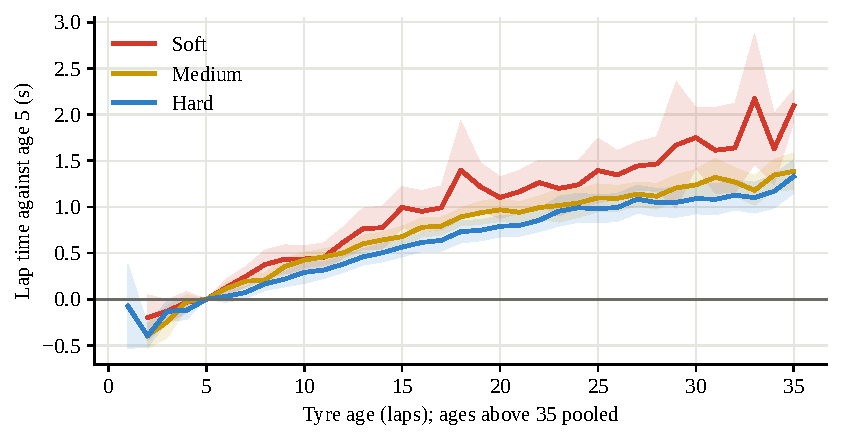
\includegraphics[width=\textwidth]{figures/f_tyre_curves.pdf}
\caption{Lap time at each tyre age relative to age 5 of the same compound, after the fixed effects of \cref{eq:fe};
shaded: 95\% intervals clustered by race. Source: \texttt{research/results/task3}.}\label{fig:curves}
\end{figure}

\paragraph{Economic reading.} The slopes put a price on keeping a set. Over a 25-lap stint, the medium tyre's slope adds
up to about 14.3\,s (that is, $0.048\times\sum_{k=0}^{24}k$) relative to a set that stayed new, and the hard about 12.7\,s,
against a pit stop that costs about 25\,s. The strategist's choice is the familiar replacement problem of capital
theory: keep a depreciating asset or pay a fixed cost to renew it \parencite{rust1987}. In a stylised version with a
linear slope $b$, a pit loss $P$ and a race of $N$ laps split into $k$ equal stints, total time lost is $bN^2/(2k)+P(k-1)$,
minimised at $k^*=N\sqrt{b/(2P)}$. With the medium slope, $P=24.9$\,s (\cref{sec:sim}) and $N=57$, $k^*\approx1.8$
stints. Because the two-compound rule requires at least two stints, the stylised optimum is a one-stop race, and a
second stop pays only when the slope exceeds $12P/N^2\approx0.09$\,s per lap, about twice the medium estimate. Real
races split almost evenly: of the 819 classified drivers who completed the full distance in the 62 dry races in the
simulator, 43.3\% stopped once and 42.2\% twice. The stylised model leaves out the faster pace loss early in a stint,
the softer compounds, safety cars and racing between cars, all of which can make a second stop worthwhile, so it is an
illustration built on the estimates, not a tested model of team behaviour. Its message is that many dry races sit close
to the margin between one stop and two.

% ----------------------------------------------------------------------- simulator
\section{The strategy simulator against real races}\label{sec:sim}

A counterfactual strategy outcome cannot be observed: no race was run twice. The simulator was therefore tested on the
parts it is built from, with every race checked using parameters estimated without it (\cref{tab:bt}).

\begin{table}[htbp]
\centering
\caption{Simulator backtest (leave-race-out parameters)}\label{tab:bt}
\begin{threeparttable}
\footnotesize
\begin{tabularx}{\textwidth}{>{\raggedright\arraybackslash}p{3.6cm}Lrrrr}
\toprule
Check & Sample & Model MAE & Model bias & Persistence MAE & Persistence bias\\
\midrule
\tabinput{tables/t_backtest.tex}
\bottomrule
\end{tabularx}
\begin{tablenotes}\footnotesize
\item \textit{Note.} Next-stint pace: clean laps after a real pit stop, forecast from just before the stop. Remaining race
time: the strategy each driver actually ran, from a decision lap at one third of the race distance, for drivers with no
safety car, virtual safety car or red flag afterwards. Positive bias: the model is too slow. Source:
\texttt{research/results/simulator}.
\end{tablenotes}
\end{threeparttable}
\end{table}

For pace on new tyres after a stop, the simulator's error is 0.876\,s per lap against 1.597\,s for repeating the last
lap before the stop, a 45\% reduction (\cref{tab:bt}). Its bias, however, is positive: it predicts fresh-tyre laps too
slow, by 0.40\,s per lap in the first three laps after a stop and by less than 0.06\,s after 30 laps (\cref{fig:nsb}).
This pattern matches the curvature found in \cref{sec:t3}: real pace changes faster early in a stint than the linear
slope assumes. Its consequence for strategy is specific: each extra stop adds a stint that starts too slow in the model,
so the simulator overcharges each additional stop by roughly 1--2\,s and leans slightly towards fewer stops.

\begin{figure}[htbp]
\centering
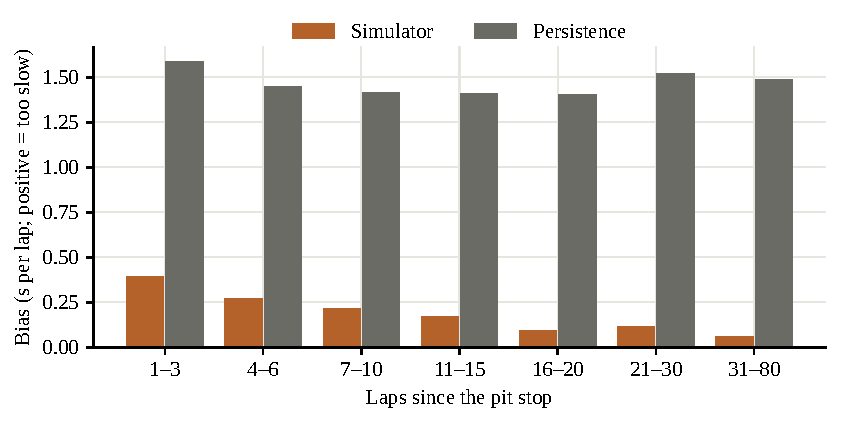
\includegraphics[width=\textwidth]{figures/f_nextstint_bias.pdf}
\caption{Bias of next-stint lap forecasts by laps since the pit stop; positive means the forecast is too slow. Source:
\texttt{research/results/simulator}.}\label{fig:nsb}
\end{figure}

Over the remaining two thirds of a race, the simulator's mean absolute error is 35.1\,s for 537 drivers in 43 races, and
it is too slow by 19.1\,s on average, about 0.5\,s per lap. Pit loss per stop is close to unbiased ($-0.88$\,s over 1,572
stops). These are errors in absolute race time and should not be read as an interval for the gap between two
strategies: much of the error, such as the driver's pace level and the per-lap trend, is shared by every plan for the
same driver and cancels when two plans are compared under common random numbers. The part that does not cancel is the
fresh-tyre bias described above.

\paragraph{Calibration.} A final check, added after the simulator was frozen and not used to change it, asked how often
the real remaining time fell inside the simulator's own ranges. It did so in 34.1\% of cases for the 50\% range and
74.3\% for the 90\% range, against 50\% and 90\% nominal. The misses are lopsided: 18.8\% of drivers were faster than the
whole 90\% range and only 6.9\% slower. Read as a risk-model backtest, this is like a 90\% value-at-risk model breached
on 25.7\% of days instead of 10\%. A Kupiec unconditional-coverage test rejects correct coverage (138 misses in 537
against 54 expected; likelihood ratio 107.5, $p<0.001$; \cite{kupiec1995,christoffersen1998}). Because nearly all misses
fall on one side, and the median 90\% range (63\,s) is wider than the typical error (35\,s), the problem is the centre
of the distribution, the +19\,s bias, rather than its width. The simulated ranges describe the uncertainty the model
knows about (parameters, driver pace, lap noise, pit-stop variation and safety cars), not its systematic error.

% ======================================================================= case study
\section{Case study: the 2024 Italian Grand Prix}\label{sec:case}

\subsection{The race}
The 2024 Italian Grand Prix at Monza was run on a circuit resurfaced for the first time since 1922
\parencite{ferrari_monza}. Teams reported graining on the new tarmac in practice \parencite{f1_monza_friday}, and Pirelli
described the graining on both compounds used as quite marked \parencite{pirelli_monza_graining}. With much of the field
expecting two stops, Ferrari kept Charles Leclerc on a one-stop strategy while McLaren stopped Oscar Piastri and Lando
Norris twice \parencite{f1_monza_race,fia_monza}. Leclerc won, 2.664\,s ahead of Piastri, whose tyres were much fresher
at the end \parencite{autosport_monza}. Norris said a one-stop had not been possible with the graining he had
\parencite{aap_monza}, and an Autosport analysis judged the one-stop marginally faster than the two-stop
\parencite{autosport_monza_analysis}. \Cref{fig:mstints} shows the stints of the leading drivers in the data.

\begin{figure}[htbp]
\centering
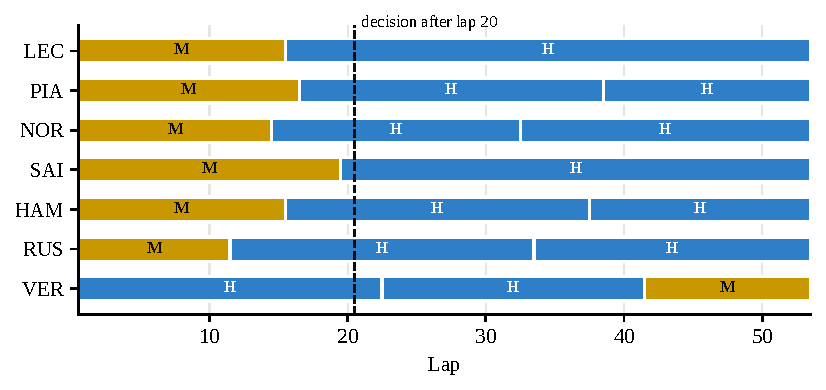
\includegraphics[width=\textwidth]{figures/f_monza_stints.pdf}
\caption{Tyre stints of selected drivers, 2024 Italian Grand Prix (S soft, M medium, H hard). The dashed line marks the
decision point used below. Source: OpenF1 stints \parencite{openf1}.}\label{fig:mstints}
\end{figure}

\subsection{The decision and the model}
After lap 20, both Leclerc and Piastri were on hard tyres after their first stop, five and four laps old respectively. With 33 laps
remaining, the question was whether to stop again for fresh tyres or to run this set to the finish. The simulator was
run from that point with every parameter estimated without this race. Its tyre-wear factor for Monza, 0.84 times the
average, came from the circuit's two other years in the sample; each driver's pace came from 17 clean laps already
run; pit loss was 25.8\,s per stop on average; and no safety car was drawn, since none occurred.

\begin{table}[htbp]
\centering
\caption{Monza 2024 from lap 20: actual plan against the alternative}\label{tab:monza}
\begin{threeparttable}
\footnotesize
\begin{tabularx}{\textwidth}{lLL>{\raggedleft\arraybackslash}p{1.7cm}l>{\raggedleft\arraybackslash}p{1.5cm}>{\raggedleft\arraybackslash}p{1.5cm}}
\toprule
Driver & Actual plan & Alternative & Alternative minus actual (s) & 90\% of races & Alternative faster (\%) & Break-even wear\\
\midrule
\tabinput{tables/t_monza.tex}
\bottomrule
\end{tabularx}
\begin{tablenotes}\footnotesize
\item \textit{Note.} 1,000 simulated races per plan with common random numbers, seed 2026. Negative: the alternative is
faster. Break-even wear: the multiplier on the model's tyre-age effect at which one stop and two stops take the same
expected time. Model-based counterfactual estimates, not observations. Source: \texttt{paper/data/monza.json}.
\end{tablenotes}
\end{threeparttable}
\end{table}

\Cref{tab:monza} gives the results. For Piastri, staying out to the finish instead of stopping a second time is
estimated to be 14.1\,s faster, with 90\% of simulated races between 6.5 and 22.0\,s faster, and faster in all 1,000. For
Leclerc, the one-stop he actually ran is the model's own best plan; adding a second stop is 10.8\,s slower on average and
faster in only 1.7\% of simulated races.

\begin{figure}[htbp]
\centering
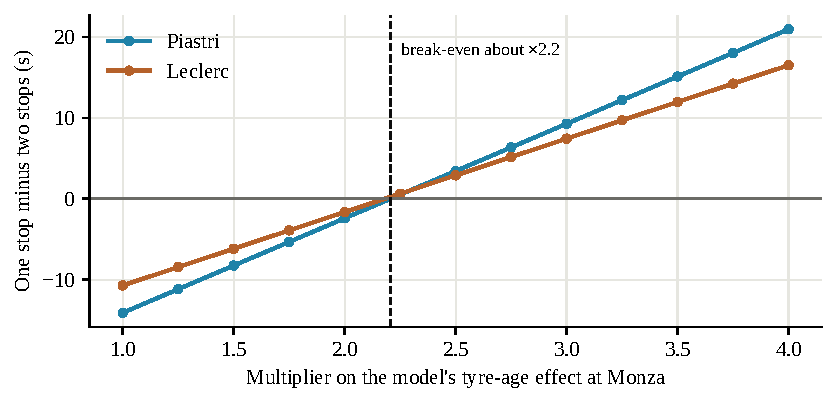
\includegraphics[width=\textwidth]{figures/f_monza_sensitivity.pdf}
\caption{Expected time of one stop minus two stops from lap 20, as the model's tyre-age effect at Monza is scaled up.
Below zero, one stop is faster. Source: \texttt{paper/data/monza.json}.}\label{fig:msens}
\end{figure}

\subsection{What can and cannot be concluded}
The model, which never saw this race, agrees with the direction of the call: one stop is preferred for both drivers,
as Ferrari decided and the published analysis judged. It overstates the size: the real race was close enough that a
two-stopping car finished 2.664\,s behind a one-stopper after a fight for position, not 14\,s. \Cref{fig:msens} shows
how much tyre wear would close that gap: two stops become faster only if the tyre-age effect at Monza was about 2.2 times
the model's estimate, for both drivers. One plausible reading, which this analysis does not test, is that the new
surface made tyres wear roughly twice as fast as the model's history of Monza implied, consistent with the reports of
graining; a model built only on earlier races could not know this before the race. Two other omissions point the same
way: the extra-stop bias of \cref{sec:sim} favours the one-stop by 1--2\,s, and the single-car model ignores the battle
between Piastri and Norris and whether a driver could actually nurse a grained set for 33 laps. The case does not show
that McLaren decided wrongly, since a team reading live tyre data had information this model lacks.

% ======================================================================= discussion
\section{Discussion}\label{sec:discussion}

\paragraph{When does added complexity stop paying?} On public timing data, the three neural networks matched
gradient-boosted trees on the next lap and fell slightly behind over ten laps, at many times the training cost. This
agrees with benchmark evidence that tree ensembles remain at least as accurate on tabular data
\parencite{grinsztajn2022,shwartzziv2022}. The design of the comparison points to a reason. The MLP saw exactly the
inputs XGBoost saw and did no better, so the learner was not the constraint. The LSTM and TCN added the raw lap
sequence and did no better than the MLP, so the hand-built summaries of recent pace already carried what the sequence
contained. What remains unexplained is the 0.33\,s typical error itself. A plausible reading, not tested here, is that
it reflects information no model sees in public data: traffic and dirty air, driver intent (pushing or saving tyres),
tyre temperatures and team instructions. In economic terms, the forecasting problem looks supply-constrained in
information, not in modelling capacity, and investment in data would likely earn more than investment in architecture.

\paragraph{What the forecasts are worth to a strategist.} The best model reduces the error over ten laps by about
1\,s, around 4\% of the cost of a pit stop. That is useful at the margin, for example when two plans are close, but it
does not transform strategy; the larger gains come from getting the structure right, such as separating tyre ageing
from fuel burn (\cref{sec:t3}). The stylised replacement model puts the average dry race near the margin between one
and two stops, and real finishers split almost evenly between the two (\cref{sec:t3}), so many decisions are close
calls where a small bias, such as the simulator's 1--2\,s per extra stop, can tip the recommendation.

\paragraph{Why measured error matters.} Simulated strategy outcomes are easy to present as facts. The calibration test
shows why they should not be: the simulator's ranges contained the real outcome far less often than claimed, mainly
because the whole distribution sat about 19\,s too slow. Comparisons between plans are more robust than absolute times,
because shared errors cancel, but the remaining strategy-specific bias should be stated next to any recommendation, as
it is on the project website.

% ======================================================================= limitations
\section{Limitations}\label{sec:limits}

\begin{itemize}
  \item \textbf{Sample.} Three seasons from one set of technical regulations and an unofficial data source
  \parencite{openf1}; one race excluded for incomplete data. Results may not carry over to a regulation change.
  \item \textbf{Test size.} Twelve test races per task. Intervals are race-clustered and therefore wide relative to the
  differences between the best models; ``equivalent'' is relative to the pre-registered margin, not a claim that the
  models are identical \parencite{lakens2017}.
  \item \textbf{Scored laps.} Accuracy refers to clean green laps; laps after stops, under neutralisation or in heavy
  traffic are not scored.
  \item \textbf{Tyre-age effect.} An association in lap time, identified from pace changes at pit stops under the
  assumptions in \cref{sec:t3method}; pit timing is chosen, so the estimates are not causal effects of wear
  \parencite{angrist2009,fosse2019}. The linear headline understates early-stint losses.
  \item \textbf{Simulator.} One car against the clock; no traffic, track position, other cars' strategies or available
  tyre sets; dry races only; virtual safety cars not modelled. Its absolute times are biased and its ranges too narrow
  for absolute outcomes (\cref{sec:sim}). The simulator was frozen before the calibration check and was not changed
  in response to it.
  \item \textbf{Case study.} One race; facts about the race come from published reports, and the interpretation of the
  gap is a plausible reading, not a test.
\end{itemize}

% ======================================================================= conclusion
\section{Conclusion}\label{sec:conclusion}

Can deep learning forecast Formula~1 lap times better than statistical and standard machine learning models? On the
evidence of a pre-registered test on twelve unseen races, not with public timing data: neural networks were equivalent
to gradient-boosted trees on the next lap and slightly behind over ten laps, at far higher cost. The largest gains came
from structure rather than complexity: separating tyre ageing from fuel burn reveals tyre-age effects of 0.04--0.07\,s
per lap that raw lap times hide. A strategy simulator built on these estimates is informative about comparisons between
plans but biased in absolute time, and its interval calibration fails; the Monza 2024 case shows both its value and its
limits. Future work should focus on information, for example gaps to other cars and tyre temperatures, and on
modelling the faster pace loss early in a stint, which the backtest identified as the simulator's main strategy-relevant
bias.

% ======================================================================= references
\newpage
\printbibliography[heading=bibintoc,title={References}]

% ======================================================================= appendix
\newpage
\appendix
\section{Reproducibility and pre-registration}\label{app:repro}

\begin{itemize}
  \item \textbf{Repository.} \url{https://github.com/NahianIbnat-2000/stint-theory}, including the pipeline, models,
  simulator, generated reports, website and this report's sources (\texttt{paper/}).
  \item \textbf{Task 1 pre-registration.} \texttt{docs/preregistration.md}, git commit
  \texttt{5c481b0f}, SHA-256 \texttt{98780c55b2eebef4\ldots}.
  \item \textbf{Task 2 pre-registration.} \texttt{docs/preregistration\_task2.md}, git commit \texttt{c662c564}, SHA-256
  \texttt{991df6177c18b37c\ldots}.
  \item \textbf{Test lock.} Test rows are removed when data are loaded unless an environment variable is set; every
  opening is written to \texttt{data/reports/test\_access.log}. The test runners refuse to start if the pre-registration
  is missing or uncommitted, or if a final report already exists.
  \item \textbf{Changes after development results.} Every change made after looking at development results is listed
  with the run that prompted it in \texttt{docs/model\_changes.md}.
  \item \textbf{Simulator parity.} The website runs a line-by-line JavaScript port of the simulator; automated tests
  check it against the Python version, draw by draw, on the exported races.
  \item \textbf{This report.} \texttt{node paper/monza.mjs}, then \texttt{python paper/make\_assets.py}, then compile
  \texttt{paper/stint\_theory\_report.tex} with XeLaTeX and Biber.
\end{itemize}

\end{document}
